%=======================================================================================%
\chapter{From Protons to Proteins: Methods to simulate the inside of a cell.}
\numberwithin{equation}{chapter}
\label{chap:methods}

\section{Quantum Mechanics is Not Tractable at the Scale of Biology.}
Living things are made of atoms and atoms themselves are composed of many particles. The motions of atoms and their constituent particles are governed by quantum mechanics. Unfortunately, performing simulations for the number of atoms involved in proteins and other cellular components at quantum mechanical accuracy is impossible. Hence, we will show how to take the fundamental formulation of atomic interactions in the Schr\"{o}dinger wave equation and apply approximations in order to produce a model which is capable of simulating macromolecular systems at biologically relevant timescales. 

We will gradually integrate upwards, beginning with the interactions in a single atom we will work our way up to a complex macromolecular system with lipids, water, salts and of course, proteins. Ultimately this section rationalises the treatment of atoms as point charges in classical molecular dynamics simulations. It is hoped that this section can be of use to both biologists and physicists, in order to teach the physicist what htey need to know about the models they will be using to perform these simulations (and the many technical problems they will encounter) and to inform the biologist what the physicist is doing with all that computer time. 

\subsection{A full quantum mechanical treatment}
Since we are dealing with atoms which are governed by quantum mechanics we must begin our journey upwards with the time dependent form of the Schr\"{o}dinger wave equation. 

\begin{equation}
i\hbar \frac {\partial}{\partial t} \Psi (\textbf{x},t) = \big[ -\frac{\hbar ^2}{2m}\nabla^2 + V (\textbf{x}, t) \big] \Psi (\textbf{x},t) 
\label {schordinger_time_dependent}
\end{equation}

In quantum systems we treat all particles as waves hence the use of the wave function $\Psi (\textbf{x},t)$. The complex amplitude of the wave function $|\Psi (\textbf {x}, t)|^2$ tells us the likelihood of detecting the particle at time $t$ and at place $\textbf{x}$. The term in the brackets correspond to $-\frac{\hbar ^2}{2m}\nabla^2 $ the kinetic energy of the particle with mass $m$ while $V (\textbf{x}, t)$ is the potential energy of the system. Given that the left hand term $i\hbar \frac {\partial}{\partial t} \Psi (\textbf{x},t)$ contains a gradient with respect to time, it governs how the wave function will evolve in time.

When the external potential $V$ has no explicit dependence on time, this equation reduces to the familiar time independent form. 

\begin{equation}
	E \Psi (\textbf{x}, t) = \big[ -\frac{\hbar ^2}{2m}\nabla^2 + V (\textbf{x}) \big] \Psi (\textbf{x}, t) = H \Psi(\textbf{x}, t) 
 \end{equation}

Note that the wave function $\Psi (\textbf {x}, t)$ is still allowed to evolve in time. 

In an atom there are two types of particles, nuclei which we will denote with the subscript $i$ and electrons denoted by $e$. In order to treat these elements separately we decompose the Hamiltonian of the system into a few components. 

\begin {equation}
H = T_n + T_e + V_{n-n} + V_{n_e} + V_{e-e}
\end{equation}

Where $T_n$ and $T_e$ denote the kinetic energy of the nucleus and electrons respectively. While $V_{n-n}, V_{n-e}, V_{e-e}$ denote the potential energy for interactions between nuclei, between electrons and nuclei and between electrons respectively.

Since the potential terms all describe charged species, they follow Coulomb's law and have the form.

\begin{equation}
	V_{n-n} = \sum_{i>j} \frac{q_e^2 z_i z_j }{|\textbf{R}_i-\textbf{R}_j|},\quad V_{n-e} = \sum_{i,l} \frac{q_e^2 z_i }{|\textbf{r}_l-\textbf{R}_i|},\quad  V_{e-e}  = \sum_{l>k} \frac{q_e^2 }{|\textbf{r}_l-\textbf{r}_k|}
\end{equation}

Here the $z_i$ represent the charge atomic number (and thus the charge) of the $i$th nucleus and $q_e$ is the unit charge of the electron. The reason for the separate coordinates $R_i$ and $r_l$ is to separate out the treatment of nuclei and electrons which will be important once we apply the Born-Oppenheimer approximation.

Meanwhile, the kinetic energy terms are quite simple. 

\begin {equation}
T_n = - \sum_i \frac{\hbar^2}{2M_i} \nabla_i ^2,\quad  T_e = - \sum_l \frac{\hbar^2}{2m_l} \nabla_l ^2
\end {equation}

$M_i$ represents the mass of the $i$th nucleon and $m_l$ represents the mass of the $l$th electron. The separate subscripts $i$ and $l$ are due to the different coordinates which we use to denote the positions of the nuclei and the electrons. The reason for this will become clear when we apply the Born-Oppenheimer approximation to separate the wave functions and solve them separately.

Here, the $M_i$ are the masses of the nuclei and the operator $\nabla = \frac{\partial}{\partial x} + \frac{\partial }{\partial y} + \frac{\partial}{\partial z} $


\subsection{The Born-Oppenheimer approximation.}
We now make use of the Born-Oppenheimer approximation \cite{Born1927}. This approximation is motivated by the observation that electrons are 3-4 orders of magnitude lighter than the nucleus, so the kinetic energy in the electrons is negligible and we can assume that the electrons will respond instantaneously to any changes in the wave function of the nucleus. Thus, we can disregard $T_e$, $U_{n-e}$ and $U_{e-e}$

This allows us to split the total wave function into two parts using a direct product. One term deals with the nuclei and one with the electrons in the system. 

\begin {equation}
\Psi(R_i,t) = \psi_e (r_l,R_i) \psi_n(R_i,t)
\end {equation}

\subsection{Simulating Molecules Without any Quantum Mechanics}
The Born-Oppenheimer approximation can be followed further to derive Hartree-Fock methods which allow calculations of the organisation of electron clouds around small molecules. This lets us derive the energy profile of certain degrees of freedom within the molecule such as the energetics of stretching out a bond or twisting a dihedral angle. 

However, even with these approximations simulating a large number of atoms is not computationally tractable. So, we must use another round of approximations to reach the spatial and time scales necessary to simulate biological molecules. We do this by creating a set of mathematical functionsthe calculations further. Here we use a set of virtual springs and other simple models for the energetic interactions between atoms. This creates what's known as an effective potential. So named because it effectively approximates the behaviour of the full quantum mechanical sytsem.

This formulation gives us classical molecular dynamics we try to match these energetic functions using an effective potential. 
The CHARMM effective potential employed in this work is common in all-atom molecular dynamics. The same  functional forms are used in other forcefields such as AMBER, GROMOS and OPLS but with different parameters and design philosophies. [CITATION NEEDED]

We split up the molecular potential into several components dealing with the energies from covalent bonds, including bond stretching, twisting and pinching. As well as energies associated with the forces that atoms exert on each other when they are not bonded together. Namely and Coulomb forces due to electric charges on the atom and attractive Van Der Walls interactions and repulsion due to Pauli Exclusion the latter two forces are combined into one term we will analyse in detail $U_{LJ}$.

\begin{equation}
	U_{CHARMM} = \underbrace{U_{LJ} + U_{Coulomb}}_{U_{non-bonded}} + \underbrace{U_{bonds} + U_{angles} + U_{dihedrals} + U_{impropers}}_{U_{bonded} + U_{Urey-Bradley}}
\end{equation}

Interestingly, the bonded terms may all reasonably be approximated by harmonic springs. 

\begin{equation}\label{bonded_eqs}
	\begin{aligned}
	U_{bonded} = \sum_{bonds} k_{b} (b-b_0)^2 + \sum_{angles} k_\theta(\theta-\theta_0)^2 + \sum_{dihedrals} k_\phi (1+\cos(n \phi - \delta)) \\ \sum_{improper-dihedrals}  k_{\kappa} (\kappa - \kappa_0)^2 + \sum_{Urey-Bradley} k_u(u-u_0)^2 
\end{aligned}
\end{equation}

Here, the $k_i$ terms correspond to the strength of the harmonic restraint for that parameter. The $0$ subscript denotes the equilibrium position for that parameter. Even though this formulation is quite simple, it has empirically been shown to accurately model the quantum energetics of bonded interactions at room temperature this can be seen in figure \ref{morse_potential}.

In classical forcefields the non-bonded interactions are expressed using the Couloumb's law because the partial charges assigned to each atom and the Lennard-Jones potential to approximate the interactions arising from both Pauli exclusion and Van Der Walls Interactions.



\begin{equation}\label{nonbonded_eqs}
	\begin{aligned}
		U_{non-bonded} = \sum_{i>j} \epsilon \Big(\frac{\sigma_{ij}}{r_{ij}}\Big)^{12} - \Big(\frac{\sigma_{ij}}{r_{ij}}\Big)^{6} - \sum_{i>j} \frac{q_i q_j } {r_{ij}}
	\end{aligned}
\end{equation}

The $\sigma$ parameter denotes the location of the local minima in the Lennard-Jones potential. This is the optimum distance that two atoms will rest against each other in the absence of other effects. The $\epsilon$ parameter denotes the depth of the potential well, or how stable the two atoms will be in the minimum energy configuration. This is very important for certain physical parameters such as osmotic pressure  \cite{Yoo2018}


\begin{figure}
	\centering
	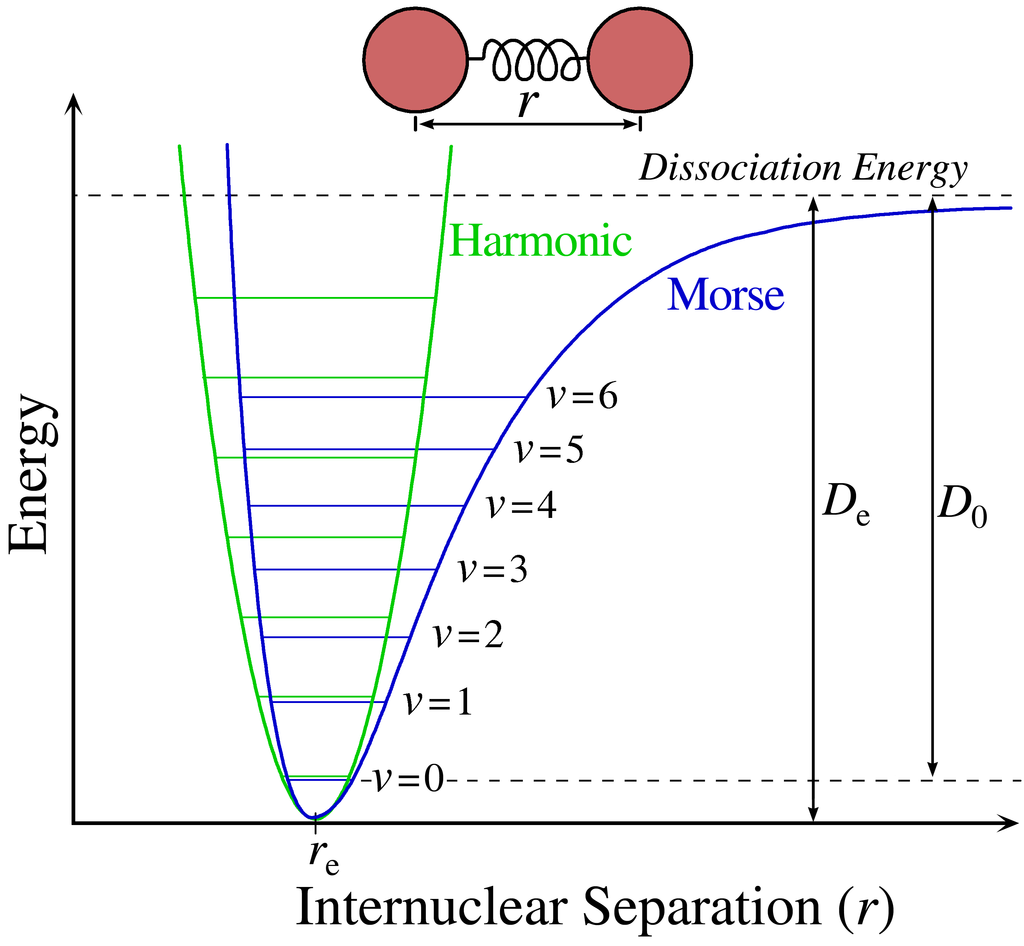
\includegraphics[width=10cm]{figures/Morse-Potential.png}
	\caption[The Morse Potential Compared to a Harmonic Potential]{
		The Morse potential was formulated to model the potential the potential energy surface of the separation of diatomic molecules (blue). At low temperatures (the ground state, v=0) like those found in classical MD there is good agreement between the Morse potential and the harmonic quantum oscillator (green). Credit Mark Somoza 2006. 
}
	\label{morse_potential}
\end{figure}


\subsection{Short Comings of Classical MD}
These approximations are not without a cost to accuracy. In certain situations, many of which are biologically relevant, it has been shown that quantum effects such as polarisation play an important role in the dynamics of the system. This has been demonstrated in the literature for Gramicidin where polarisable forcefields are able to more accurately reproduce the experimental results of current.
